%
% File acl2017.tex
%
%% Based on the style files for ACL-2015, with some improvements
%%  taken from the NAACL-2016 style
%% Based on the style files for ACL-2014, which were, in turn,
%% based on ACL-2013, ACL-2012, ACL-2011, ACL-2010, ACL-IJCNLP-2009,
%% EACL-2009, IJCNLP-2008...
%% Based on the style files for EACL 2006 by 
%%e.agirre@ehu.es or Sergi.Balari@uab.es
%% and that of ACL 08 by Joakim Nivre and Noah Smith

\documentclass[11pt,a4paper]{article}
\usepackage{acl2017}
\usepackage{times}
\usepackage{latexsym}

% House Style
\usepackage{booktabs}

% Other Style
\usepackage{amsmath}
\usepackage{graphicx}
\usepackage{subfig}
\usepackage{algorithm}
\usepackage[noend]{algpseudocode}

\usepackage{url}

%\aclfinalcopy % Uncomment this line for the final submission
%\def\aclpaperid{***} %  Enter the acl Paper ID here

%\setlength\titlebox{5cm}
% You can expand the titlebox if you need extra space
% to show all the authors. Please do not make the titlebox
% smaller than 5cm (the original size); we will check this
% in the camera-ready version and ask you to change it back.

\newcommand\BibTeX{B{\sc ib}\TeX}

\title{The Coadaptation Problem when \\ Learning How and What to Compose}

\author{Andrew Drozdov \\
  New York University \\
  Department of Computer Science \\
  {\tt apd283@nyu.edu} \\\And
  Samuel Bowman \\
  New York University \\
  Department of Data Science / Department of Linguistics \\
  {\tt bowman@nyu.edu} \\}

\date{}

\begin{document}
\maketitle
\begin{abstract}
This paper discusses a potential problem with tree-sequence models that induce syntax,
in that there exists a failure mode when naively treating the relationship between composition and parsing.
The first section presents a tree-sequence model that induces syntax.
The second section proposes a strategy that attempts to prevent coadaptation between composition
and parsing. The third section covers a method for randomly sampling binary trees in a transition-based
setting, a simple and useful technique for transition-based parsing models.
\end{abstract}

\section{Introduction}

The Stacked-augmented Parser-Interpreter Neural Network (SPINN) from \citet{bowman2016fast} is a hybrid tree-sequence model that uses Recursive Neural Networks \citep{socher2011parsing} with TreeLSTM composition units \citep{tai2015improved} to leverage syntactic information for semantic classification tasks. Recent work \citep{yogatama2016learning} has modified SPINN to induce a projective binary structure over its input sentence using signal from the classification task as a reward for a parsing component optimized with the REINFORCE algorithm \citep{williams1992simple}. The tree structures in \citet{yogatama2016learning} are observed to be almost trivial in nature, completely left or right leaning, rarely recovering linguistically inspired structure. This trivial behavior resembles similar behavior to a failure mode of the parser when composition becomes too strongly tied (coadapts) to a type of parse tree structure.

If the coadaptation problem is a true problem, it happens when the composition is exposed to many similar looking parse trees consecutively during training time. During evaluation time, any unseen parse tree would provide significant noise to composition. In turn, the semantic classification task becomes unnecessarily difficult. Similarly, switching parsing strategies abruptly during training can confuse composition, inhibiting downstream task performance until composition adjusts to the new strategy.

In lieu of a perfect parsing strategy during train time (or simply having labeled data), one potential method to prevent composition from coadapting to any parsing strategy is to observe as many trees for a given set of data as possible. This can be done by uniformly sampling over valid parse trees for each input. It might be helpful to still greedily parse any input to benefit semantic classification. When doing so it might help to inhibit the learning of the parser so that is more influenced by successfully randomly sampled structure rather than the biased greedy and potentially trivial structure.

Using SPINN with REINFORCE is descibed in section 2. The schedule used to randomly sample trees and modify the magnitude of gradient updates to the parser is called Soft Wake Sleep and is described in section 3. An algorithm for uniformly sampling binary trees in a transition-based parser is covered in section 4.

% Citations  \citet{bowman2016fast,yogatama2016learning,dyer2016rnng,rennie2016self,williams1992simple}



\section{SPINN + REINFORCE}

We use a version of the thin stack algorithm from \citet{bowman2016fast} akin to what is done in \citet{yogatama2016learning}. \footnote{Code published on github. Left out for anonymous submission.}

Our initial experiments with SPINN in this setting unveiled two problematic circumstances:

\begin{enumerate}
\item
The model commonly follows parsing behavior that returns strictly left or right branching trees (similar behavior was seen in \citet{yogatama2016learning}).
\end{enumerate}

\begin{enumerate}
\item[2]
When the parser in SPINN becomes fixated in its parsing
strategy for a significant number of examples, the composition function coadapts with the parsing behavior.
\end{enumerate}

For these reasons, it's highly desirable to prevent coadaptation
because an unprepared compositional function propogates noise throughout the model, making
classification difficult and exploring non-trivial tree structures too costly.

In the following section we detail a training strategy that attempts to prevent coadaptation
and ease the exploration of substructures.

\section{Soft Wake Sleep}

To interpolate between training the parser and the composition function, we apply
temperature to the softmax layer of the transition network defined by an annealed
sinusoidal schedule (as seen in Figure~\ref{fig:schedule}). We apply a similar temperature to scale the loss of the transition
network.

	When $T$ is large ($>1$), the distribution for sampling binary trees is most random. Simultaneously, $\rho$
will be high and the parser will be most effected by gradient updates. When $T$ is small ($<1$), the parser will sample binary trees from a more greedy-like distribution and the parser will be less effected by updates.
This periodic behavior encourages the composition function to act reasonably over many different tree structures,
and discourages the parser from becoming fixated in a trivial parsing strategy.

Adding temperature to the softmax is done by dividing the input of the softmax by a variable
$T$. The output of the softmax resembles a uniform distribution when $T\to\infty$.

\begin{align}
\sigma(\frac{\vec{x}}{T}) = \frac{e^{\frac{x}{T}}}{\Sigma_{\hat{x} \in \vec{x}} e^{\frac{\hat{x}}{T}}}
\end{align}

%%
% Supervised Loss
\begin{algorithm}[H]
\caption{Supervised Model}\label{loss}
\begin{algorithmic}[1]

\Function{Model}{sentences, transitions, y}
\State Ts := transitions.T
\State outp, Ts$'$ := \Call{SPINN}{sentences, Ts}
\State y$'$ := $f^y$(outp)
\State Loss$_y$ := \Call{NLL}{y, y$'$}
\State Loss$_T$ := \Call{NLL}{Ts, Ts$'$}
\State \Return Loss$_y$, Loss$_T$
\EndFunction

\end{algorithmic}
\end{algorithm}

%%
% Supervised SPINN
\begin{algorithm}[H]
\caption{SPINN}\label{spinn}
\begin{algorithmic}[1]

\Function{SPINN}{sentences, Ts}
\State bufs := \{[$\vec{0}$] + s.reverse() $\vert$ s $\in$ sentences\}
\State stacks := \{[$\vec{0}$,$\vec{0}$] $\vert$ s $\in$ sentences\}
\State Ts$'$ := transitions.T
\For {ts $\in$ transitions}
 \State ts$'$ := \Call{BatchStep}{bufs, stacks, ts}
 \State Ts$'.push$(ts$'$)
 \EndFor
 \State \Return stacks[-1], Ts$'$
 \EndFunction

\Function{BatchStep}{bufs, stacks, ts}
\State inp := [bufs[-1], stacks[-1], stacks[-2]]
\State ts$'$ := $f^P$($f^T$(inp))
\State ts$'$ := \Call{Validate}{ts, ts$'$}
\State R, S := \Call{Distribute}{ts$'$, bufs, stacks}
\State \Call{Reduce}{R}; \Call{Shift}{S}
\State \Return ts$'$
\EndFunction

\Function{Distribute}{ts, bufs, stacks}
\State R, S $:= $ [], []
\For {t, S, Q $\in$ ts, bufs, stacks}
\If {$t = \text{REDUCE}$}
\State R$.push$(Q.pop(), S, Q)
\ElsIf {$t = \text{SHIFT}$}
\State right, left $:=$ S.pop(), S.pop()
\State S.$push$([left, right], S, Q)
\EndIf
\EndFor
\State \Return R, S
\EndFunction

\Function{Reduce}{R}
\State [lefts, rights], bufs, stacks := R.T
\State inp = [lefts, rights]
\State outp = split($f^C$(inp))
\For {o $\in$ outp, S $\in$ stacks}
\State S$.push$(o)
\EndFor
\EndFunction

\Function{Shift}{S}
\For {top, S, Q $\in$ S}
\State S$.push$(top)
\EndFor
\EndFunction

\end{algorithmic}
\end{algorithm}

% TODO:
% - Use distribution of transitions as input for reinforce
% - Use baseline

%%
% RL Loss
\begin{algorithm}[H]
\caption{Reinforce Model}\label{rlloss}
\begin{algorithmic}[1]

\Function{Model}{sentences, transitions, y}
\State Ts := transitions.T
\State outp, Ts$'$ := \Call{SPINN}{sentences, Ts}
\State y$'$ := $f^y$(outp)
\State Loss$_y$ := \Call{NLL}{y, y$'$}
\State Loss$_{RL}$ := \Call{Reinforce}{Ts$'$, Loss$_y$}
\State \Return Loss$_y$, Loss$_{RL}$
\EndFunction

\end{algorithmic}
\end{algorithm}

% Distribution Balanced Image
\begin{figure}[H]
\centering
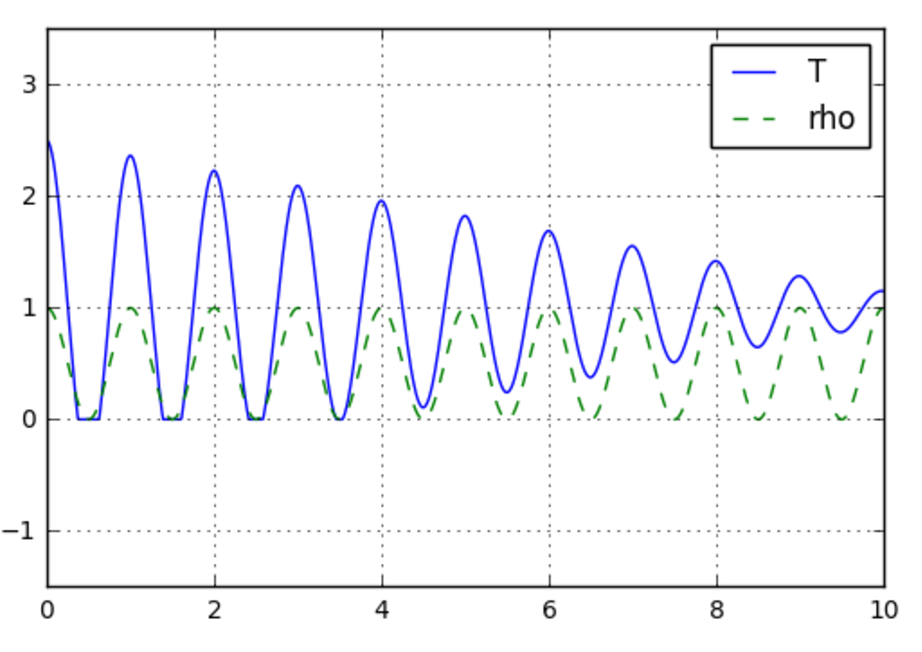
\includegraphics[width=7cm]{temperature_schedule}
\caption{The temperature T used to interpolate between greedy and random distributions when sampling transitions follows a strictly positive sinusoidal wave with annealed magnitude. The scale $\rho$ on the REINFORCE loss follows a similar schedule but is not annealed.}
\label{fig:schedule}
\end{figure}

\begin{figure}[H]
\centering
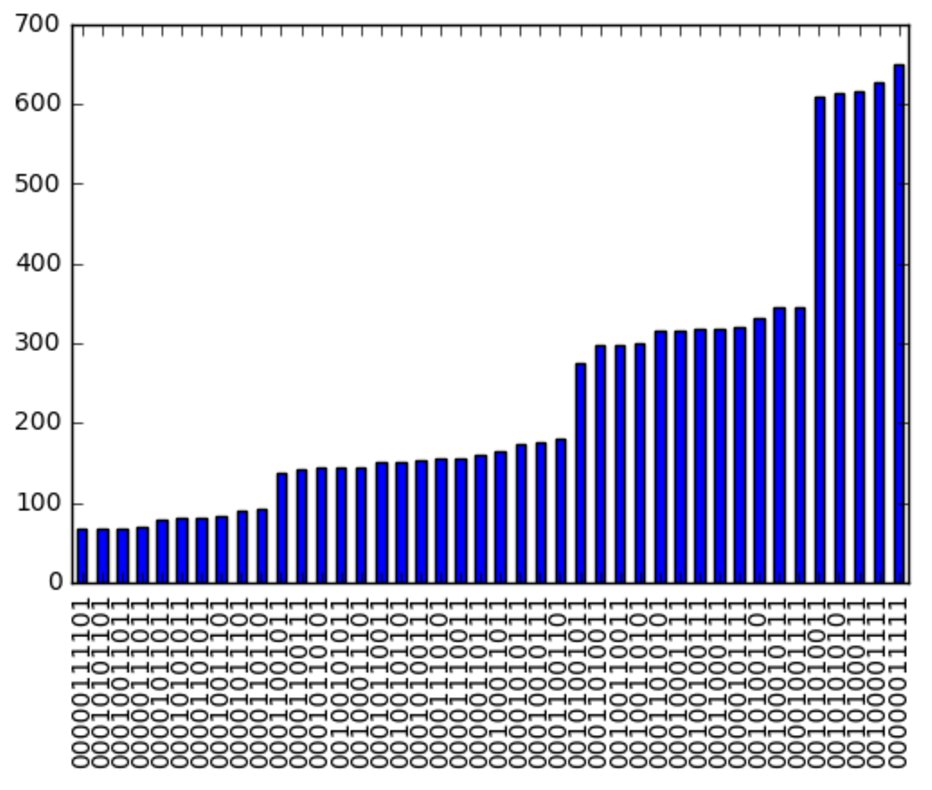
\includegraphics[width=7cm]{distribution_step}
\caption{Sampling uniformly 10k times results in frequencies that resemble a step function. Trees are represented as 0s (Shift) and 1s (Reduce).}
\label{fig:notuniform}
\end{figure}

\begin{figure}[H]
\centering
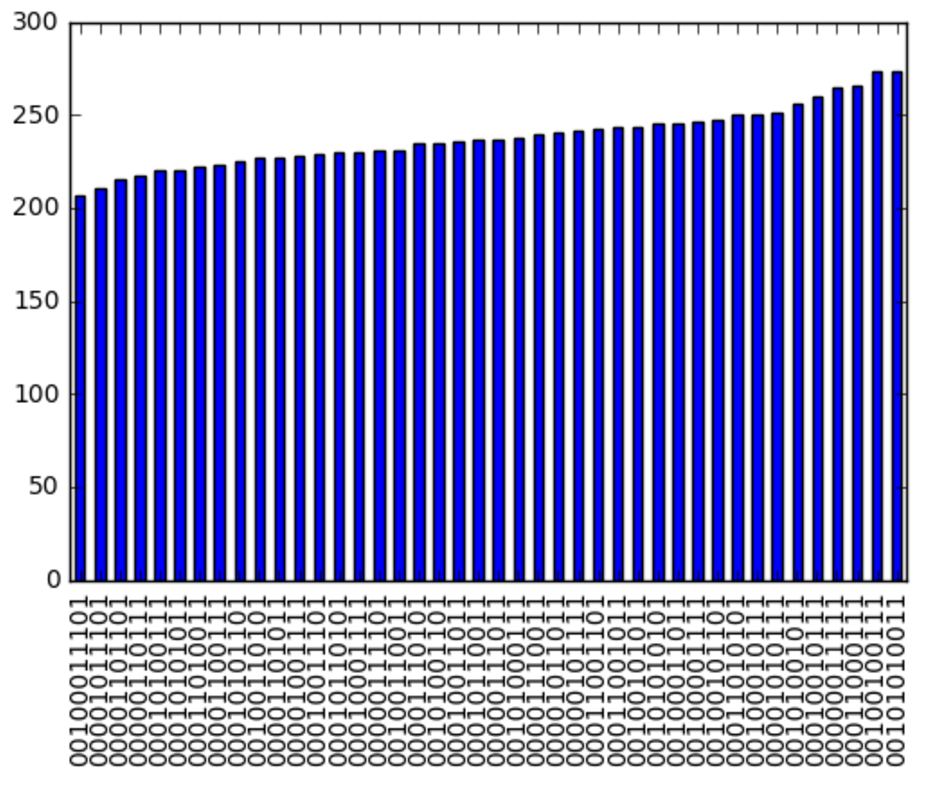
\includegraphics[width=7cm]{distribution_balanced}
\caption{Sampling from the Catalan Pyramid results in a smoother distribution of frequencies.}

% Frequency counts of randomly generated binary trees with N=6 leaves by using the a uniform distribution over Shift/Reduce transitions and the distribution from the Catalan Pyramid for Shift/Reduce transitions in sequence over 10k samples.}
\label{fig:uniform}
\end{figure}



% Distribution Step/Catalan Image
% \begin{figure}[tbp]
%   \centering
%   \subfloat[Uniformly Random]{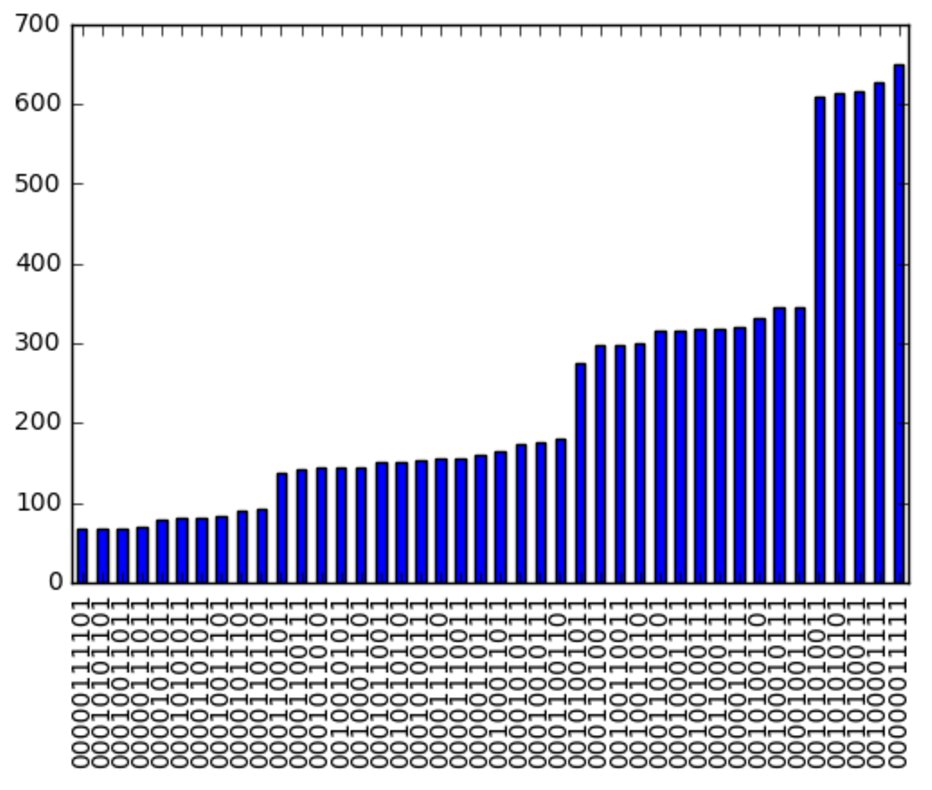
\includegraphics[width=0.2\textwidth]{distribution_step}\label{fig:f1}}
%   \hfill
%   \subfloat[Catalan Pyramid]{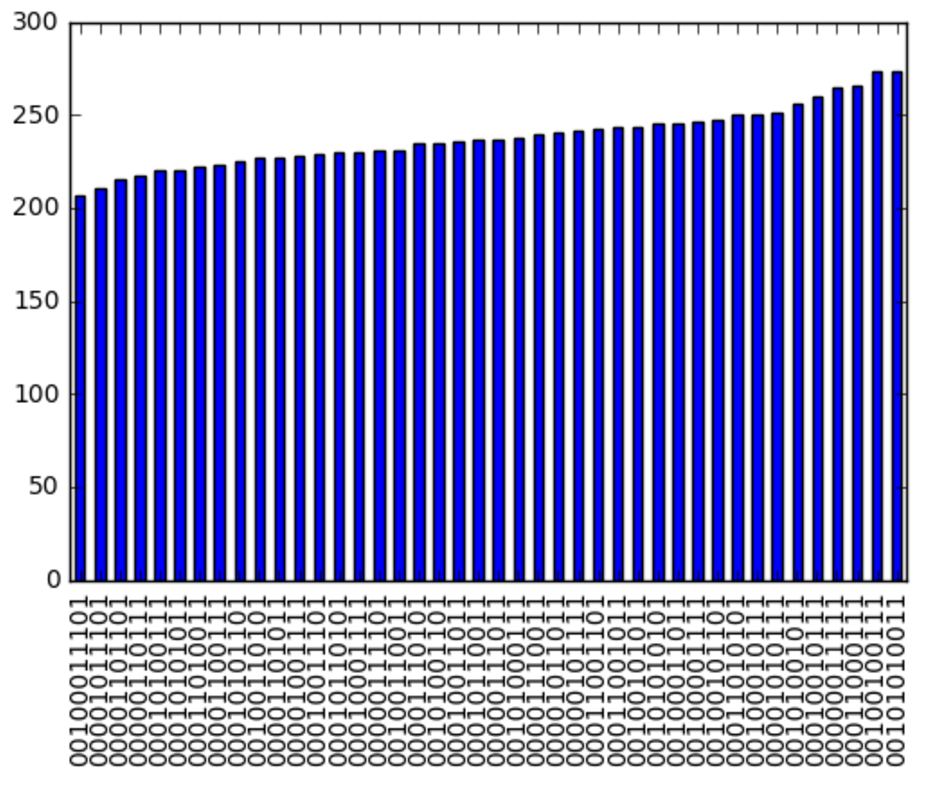
\includegraphics[width=0.2\textwidth]{distribution_balanced}\label{fig:f2}}
%   \caption{Frequency counts of randomly generated binary trees with N=6 leaves by using the a uniform distribution over Shift/Reduce transitions and the distribution from the Catalan Pyramid for Shift/Reduce transitions in sequence over 10k samples.}
% \end{figure}

% TEXT TEXT TEXT TEXT TEXT TEXT TEXT TEXT TEXT TEXT TEXT TEXT TEXT TEXT TEXT TEXT TEXT TEXT TEXT TEXT TEXT TEXT TEXT TEXT

% Catalan Pyramid
\begin{figure*}[t]
\small
\centering
\begin{tabular}{|r|l|l|l|l|l|l|l|l|l|l|l|l|l|l|l|}
\hline & t=0 & 1 & 2 & 3 & 4 & 5 & 6 & 7 & 8 & 9 & 10 & 11 & 12 & 13 & 14 \\ \hline
r=0 & 1 & 1 & $\frac{297}{429}$ & $\frac{165}{297}$ & $\frac{75}{165}$ & $\frac{27}{75}$ & $\frac{7}{27}$ & $\frac{1}{7}$ &   &   &   &   &   &   &   \\
1 &   &   &   & 1 & $\frac{90}{132}$ & $\frac{48}{90}$ & $\frac{20}{48}$ & $\frac{6}{20}$ & $\frac{1}{6}$ &   &   &   &   &   &   \\
2 &   &   &   &   &   & 1 & $\frac{28}{42}$ & $\frac{14}{28}$ & $\frac{5}{14}$ & $\frac{1}{5}$ &   &   &   &   &   \\
3 &   &   &   &   &   &   &   & 1 & $\frac{9}{14}$ & $\frac{4}{9}$ & $\frac{1}{4}$ &   &   &   &   \\
4 &   &   &   &   &   &   &   &   &   & 1 & $\frac{3}{5}$ & $\frac{1}{3}$ &   &   &   \\
5 &   &   &   &   &   &   &   &   &   &   &   & 1 & $\frac{1}{2}$ &   &   \\
6 &   &   &   &   &   &   &   &   &   &   &   &   &   & 1 &   \\
\hline
\end{tabular}
\caption{Catalan Pyramid. Represents probability of predicting shift at timestep t given there have already been r reduces.}
\label{tab:catalan}
\end{figure*}

\section{Catalan Pyramid}

Iteratively uniformly sampling transitions does not lead to uniforming sampling over binary trees in Shift Reduce Transition Based Parsing. Rather, the distribution of trees resembles a step function as seen in Figure~\ref{fig:notuniform}, which shows the frequency counts of binary trees over iterative random samples. To uniformly sample over binary trees, it's necessary to sample from a distribution representing the number of valid paths containing either Shift or Reduce as the next transition, and results in a smoother plot of frequency counts (Figure~\ref{fig:uniform}). A naive algorithm can come up with this distribution in exponential time by enumerating all possible trees of a given length, and filtering to relevant trees, but this approach is unusuable for trees with even a moderate number leaves. Fortunately, this distribution seems to have a closed form solution which can be recovered in linear time for any transition in any binary tree, and amortized constant time. We present the recursive algorithm in the following subsection and call the related distribution the Catalan Pyramid (Table~\ref{tab:catalan}) as each row contains fractions over the Catalan Numbers (which represent the count of binary trees with N leaves). A quick search did not turn up previous strategies for sampling uniformly over binary trees in transition based parsing.

\subsection{Algorithm}

For a sequence with N tokens, N*2 - 1 transitions, and N - 1 reduce transitions, can build a so-called ``Catalan Pyramid'' (Table~\ref{tab:catalan}) using these 6 rules:

\begin{enumerate}
\item
$row_{i,0,0} = 1$
\item
$row_{i,0,1} = i + 2$
\item
$row_{i,n_i-1,1} = Catalan(i + 2)$
\item
$row_{i,n_i-1,0} = row_{i,n_i-1,1} - row_{i-1,n_i-2,1}$
\item
$row_{i,j,0} = row_{i,j-1,1}$
\item
$row_{i,j,1} = row_{i,j,0} + row_{i-1,j,1}$
\end{enumerate}

These rules will build the non-zero fractions in each row of the table (0=numerator, 1=denominator), then padding the fractions as show with zeros will give you the probability of SHIFTing given that you are at timestep $t$ and have already REDUCEd $r$ times.

\subsection{Linear Interpolation of Probabilities}

The distribution from the Catalan Pyramid is not uniformly random at each time step, so the formula for temperature must be adjusted to take the proper distribution into account. Since temperature leads to a uniform distribution at its limit, it is a linear interpolation of the distribution based purely on the logits ($T = 1$) and the uniform distribution. We can recover the linear parameter directly to perform a similar interpolation between any distribution, including the one from the Catalan Pyramid.

\begin{align}
\sigma(\frac{\vec{x}}{T}) &= i \cdot \sigma(\vec{x}) + (1 - i) \cdot \sigma(0) \\
i &= \frac{\sigma(\frac{\vec{x}}{T}) - \sigma(0)}{\sigma(\vec{x})}
\end{align}


\section*{Acknowledgments}

Left out for anonymous submission.

% \newpage

% include your own bib file like this:
%\bibliographystyle{acl}
%\bibliography{acl2017}
\bibliography{acl2017}
\bibliographystyle{acl_natbib}

\end{document}
